%
% © 2009 Michael Stapelberg
%
% 2009-06-24
%
\documentclass[mode=print,paper=screen,style=jefka]{powerdot}
\usepackage[utf8]{inputenc}
\usepackage{graphicx}
\usepackage{float}
\usepackage{ngerman}
\usepackage{url}
\usepackage{listings}
\newcommand{\bs}{\textbackslash}
\pdsetup{palette=white}
\definecolor{darkblue}{rgb}{0,0,.6}
\definecolor{darkred}{rgb}{.6,0,0}
\definecolor{darkgreen}{rgb}{0,.6,0}
\definecolor{darkgray}{gray}{.3}
\definecolor{lightblue}{rgb}{0.97,0.99,1}

\lstloadlanguages{C}
\lstdefinestyle{colors}{keywordstyle={\bf\color{darkblue}}, commentstyle={\em\color{magenta}}, stringstyle={\color{darkred}},%
                        emphstyle={\color{darkgray}}}
\lstnewenvironment{code}{%
        \lstset{frame=single, basicstyle=\footnotesize\ttfamily, language=C, showstringspaces=false,%
                style=colors, numbers=left, morekeywords={xcb_get_window_attributes_cookie_t, xcb_map_request_event_t,%
                xcb_connection_t, xcb_get_window_attributes_reply_t, window_attributes_t, xcb_intern_atom_cookie_t,%
                xcb_intern_atom_reply_t, xcb_atom_t, uint32_t, uint16_t, foreach, UINT_MAX, NULL},%
                moreemph={xcb_get_window_attributes_reply, xcb_get_window_attributes_unchecked, manage_window,%
                add_ignore_event, xcb_intern_atom, xcb_intern_atom_reply, fprintf, printf, free, load_configuration,%
                XInternAtom, exit, strlen, xcb_change_window_attributes, xcb_event_wait_for_event_loop,%
                xcb_event_set_key_press_handler, xcb_property_set_handler}}
}{}

\newcommand{\isrc}[1]{\begin{center} \footnotesize\ttfamily Siehe auch: #1 \end{center}}

\title{Hacking your own window manager}
\author{sECuRE auf der GPN 8\\
~\\
powered by \LaTeX, of course}
\begin{document}
\maketitle

\begin{slide}{Dieser Vortrag}
\begin{list}{$\bullet$}{\itemsep=.5em}
        \item Geschichte/Einführung in Window Manager
        \item Merkmale von i3
        \item Window Manager und X11
        %
        % zuerst: wie funktioniert ein client?
        %
        % WM ist nur ein weiterer Client
        % Keine Rechteverwaltung, prinzipiell darf jeder Fenster schubsen
        % Clients können Events abfangen, der WM macht das halt für das root-fenster
        \item Arbeitsumgebung
        \item XCB
        \item Setup
        \item Reparenting (Window Decorations)
        %\item fake\_configure\_notify
        %\item Colorpixel
        %\item UTF-8
        % irgendwo da erwähnen: fenster in eine hashtable aufnehmen

        \item Events
        % (die kriegt man natürlich nur wenn man redirectmask gesetzt hat:)
        % MapRequest
        % ConfigureRequest
        \item Hints (Titel, Klassen, Größen, …)
        % Atoms
        % NetWM
        % - NET_WM_WINDOW_TYPE
        % - NET_WM_NAME
        %   - in kombination mit NET_SUPPORTING_WM_CHECK auf dem rootfenster
        % - NET_WM_STRUT_PARTIAL
        % ICCCM
        % - Normal hints / size hints (warum zwei namen?)
        %   - Aspect ratio, wichtig z.B. für mplayer
        %   - min/max size, interessant primär für floating
        % - WM_NAME
        % - WM_TRANSIENT_FOR
        % - WM_CLASS
        \item Gotchas
        % flush()
        % WM_STATE_NORMAL und drag&drop in gtk-apps
        \item Zusammenfassung
        % TODO
\end{list}
\end{slide}

\begin{slide}{Geschichte/Einführung}
\begin{list}{$\bullet$}{\itemsep=1em}
        \item<1-> „All window managers suck, this one just sucks less”?
        \item<2-> Desktop environment vs. window manager (GNOME, KDE, Xfce, …)
        \item<3-> Stacking (e17, fluxbox, IceWM, fvwm, …) vs Tiling (dwm, wmii, xmonad, …)
        \item<4-> dwm, awesome, xmonad, …: statisches Layout
        % gedanke: man braucht sich nicht mal mehr um das layout kümmern
        \item<5-> wmii, ion: dynamisches layout
        \item<6-> Probleme an ion: tuomov (Lizenz, Kommunikation), Config, Look and feel, Code
        \item<7-> Probleme an wmii: Xinerama-support, Xlib, undokumentierter Code, nur Spalten, keine Reihen, Kleinigkeiten (titellose Fenster)
\end{list}
\end{slide}

\begin{slide}{Merkmale von i3}
\begin{list}{$\bullet$}{\itemsep=1em}
        \item<1-> gut lesbarer, dokumentierter Code. Dokumentation.
        \item<2-> XCB anstelle von Xlib
        \item<3-> Xinerama done right™
        \item<4-> Spalten und Zeilen, Tabelle als Basis
        \item<5-> command-mode, wie in vim
        \item<6-> UTF-8 clean
        \item<7-> kein Antialiasing, schlank und schnell bleiben
\end{list}
\end{slide}

\begin{slide}{Typische Kommunikation mit X}
\begin{list}{$\bullet$}{\itemsep=1em}
        \item<1-> Verbindung aufbauen
        \item<2-> Requests über die Leitung schicken (Fenster erzeugen)
        \begin{list}{$\bullet$}{\itemsep=1em}
                \item Cookie für jeden Request
                \item Antwort für spezifisches Cookie abholen
                \item $\Rightarrow$ Asynchronität nutzbar
        \end{list}
        \item<3-> Eventloop starten, reagieren (Fenster zeichnen, Eingaben, …)
\end{list}
\end{slide}

\begin{slide}{Was genau macht ein WM?}
\begin{list}{$\bullet$}{\itemsep=1em}
        \item<1-> Events umlenken
        \item<2-> Neue Fenster anzeigen/positionieren (MapRequest)
        \item<3-> Titelleisten malen (reparenting)
        \item<4-> Den Fokus verwalten
        \item<5-> Mit Hints umgehen (Fenstertitel, Fullscreen, Dock, …)
        \item<6-> Auf Benutzereingaben reagieren
\end{list}
\end{slide}


\begin{slide}[method=direct]{Window Manager und X11 (1)}
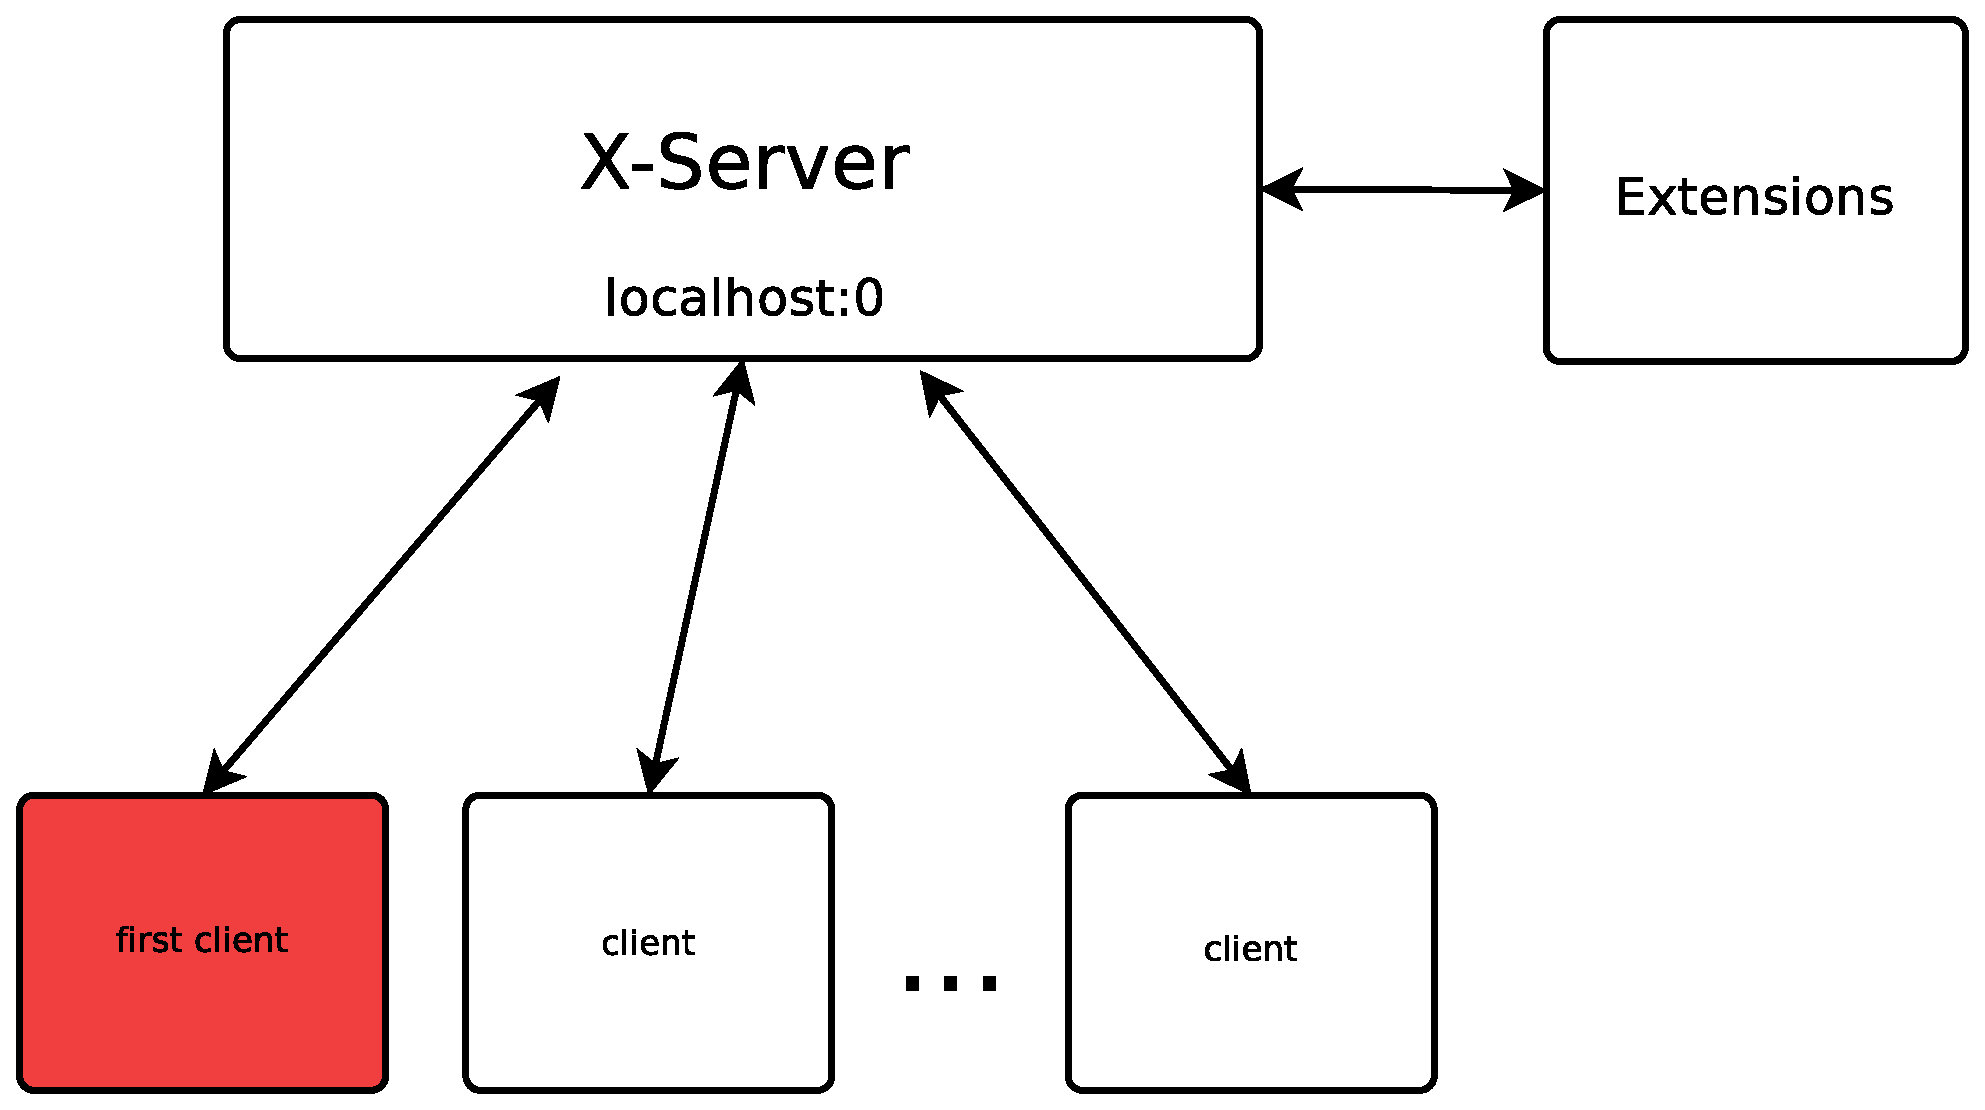
\includegraphics[width=1\textwidth]{xserver_konzept.eps}
\end{slide}

\begin{slide}{Window Manager und X11 (2)}
\begin{list}{$\bullet$}{\itemsep=1em}
        \item<1-> Keine Rechteaufteilung, prinzipiell kann jeder Fenster managen
        \item<2-> Window Manager verantwortlich für alle Kinder das Root-Fensters
        \item<3-> RedirectMask, lässt sich Events des Root-Fensters schicken
        \item<4-> Setzt hints auf dem Root-Fenster
\end{list}
\end{slide}

\begin{slide}{Arbeitsumgebung}
\begin{list}{$\bullet$}{\itemsep=1em}
        \item X sinnvoll beim Entwickeln $\Rightarrow$ anderen Computer verwenden oder Xephyr
        \item xtrace dazwischenschalten (sowohl zwischen WM und X11 als auch zwischen Clients und X11 sinnvoll)\\
\texttt{DISPLAY=:1 xtrace -o /tmp/xtrace.log -n :9}
        \item \texttt{xprop} zeigt Hints an, \texttt{xwininfo} gibt Struktur aus
        \item als ersten Client ein Terminal starten $\Rightarrow$ wenn der WM crashed lebt
        die X-Session noch\\
\texttt{DISPLAY=:1 urxvt \&}
        \item Debugger, strace, logfiles, core-dumps aktivieren\\
        (Siehe auch \url{http://i3.zekjur.net/docs/debugging.html})
\end{list}
\end{slide}

\begin{slide}{XCB}
\begin{list}{$\bullet$}{\itemsep=1em}
        \item \url{http://xcb.freedesktop.org/}
        \item<1-> „X-protocol C-language Binding”
        \item<2-> Klein, wartbar (aus einer Protokollbeschreibung auto-generiert)
        \item<3-> Sinnvoll benannte Funktionsnamen und Datentypen
        \item<4-> Nutzt die Asynchronität von X aus
        \item<5-> Allerdings: Sehr spärlich dokumentiert, man muss mit Xlib-Doku arbeiten
        \item<6-> xcb-util: XCB noch mal ein bisschen gekapselt, nützliche Funktionen abstrahiert
\end{list}
\end{slide}

\begin{slide}[method=direct]{Xlib-Beispielcode}
\begin{code}
  char *names[10] = {"_NET_SUPPORTED", "_NET_WM_STATE",
  "_NET_WM_STATE_FULLSCREEN", "_NET_WM_NAME" /* ... */};
  Atom atoms[10];

  /* Get atoms */
  for (int i = 0; i < 10; i++) {
    atoms[i] = XInternAtom(display, names[i], 0);
  }
\end{code}
\end{slide}

\begin{slide}[method=direct]{XCB-Beispielcode}
\begin{code}
char *names[10] = {"_NET_SUPPORTED", "_NET_WM_STATE",
  "_NET_WM_STATE_FULLSCREEN", "_NET_WM_NAME" /* ... */};
xcb_intern_atom_cookie_t cookies[10];

/* Place requests for atoms as soon as possible */
for (int c = 0; c < 10; c++)
  cookies[c] = xcb_intern_atom(connection, 0,
                               strlen(names[c]), names[c]);

/* Do other stuff here */
load_configuration();

/* Get atoms */
for (int c = 0; c < 10; c++) {
  xcb_intern_atom_reply_t *reply =
    xcb_intern_atom_reply(connection, cookies[c], NULL);
  if (!reply) {
    fprintf(stderr, "Could not get atom\n");
    exit(-1);
  }
  printf("atom has ID %d\n", reply->atom);
  free(reply);
}
\end{code}
\end{slide}

\begin{slide}[method=direct]{Setup}
\begin{code}
get_atoms();

xcb_event_set_key_press_handler(&evenths, handle_key_press, NULL);
xcb_property_set_handler(&prophs, WM_TRANSIENT_FOR, UINT_MAX,
                         handle_transient_for, NULL);

xcb_grab_key(conn, 0, root, modifier, keycode,
             XCB_GRAB_MODE_SYNC, XCB_GRAB_MODE_ASYNC);
xcb_grab_key(conn, 0, root, modifier | xcb_numlock_mask, keycode,
             XCB_GRAB_MODE_SYNC, XCB_GRAB_MODE_ASYNC);

uint32_t values[] = { XCB_EVENT_MASK_SUBSTRUCTURE_REDIRECT |
                      XCB_EVENT_MASK_STRUCTURE_NOTIFY |
                      XCB_EVENT_MASK_PROPERTY_CHANGE |
                      XCB_EVENT_MASK_ENTER_WINDOW };
xcb_change_window_attributes(conn, root, XCB_CW_EVENT_MASK, values);

manage_existing_windows();

xcb_event_wait_for_event_loop(&evenths);
\end{code}

\isrc{i3/src/mainx.c:370ff}
\end{slide}

\begin{slide}[method=direct]{Reparenting}
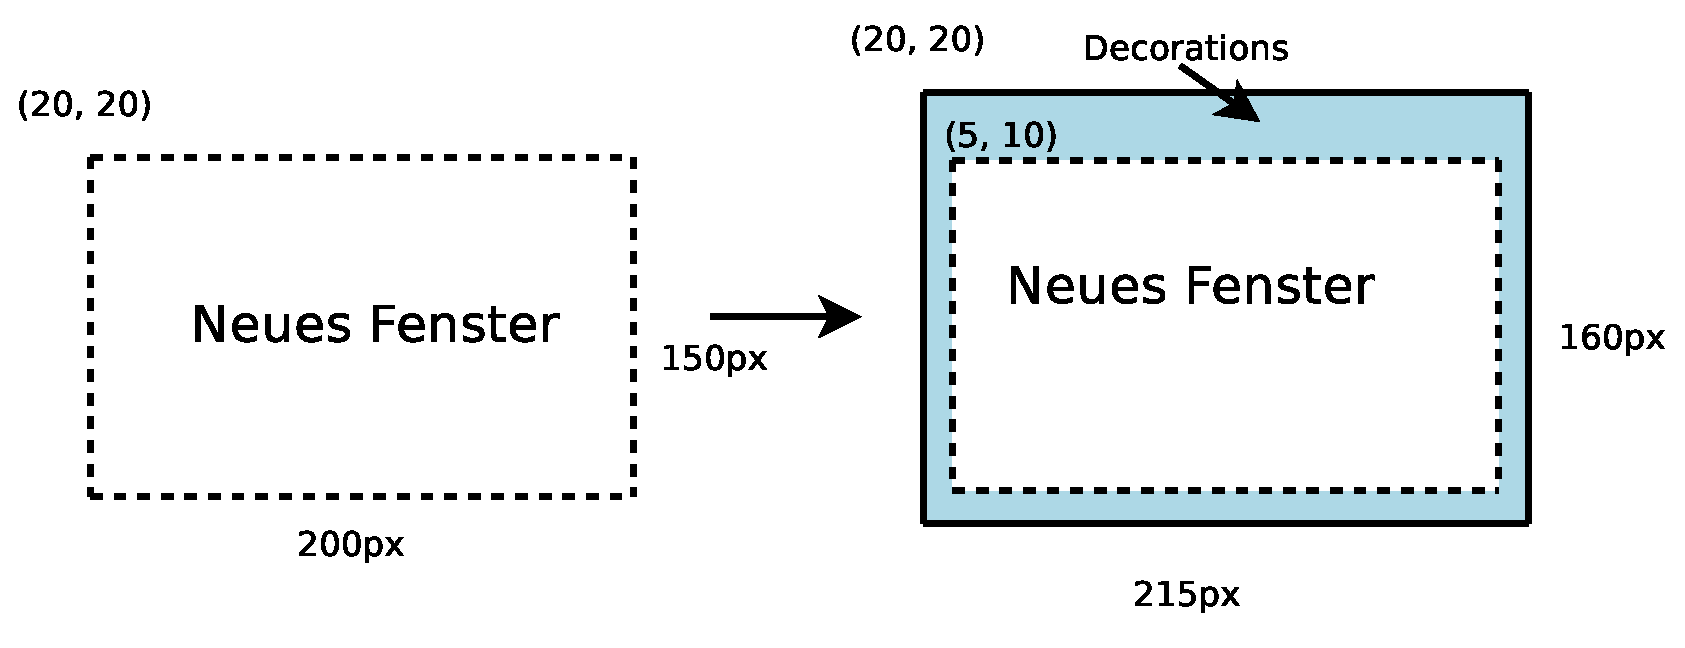
\includegraphics[width=1\textwidth]{reparenting.eps}
\begin{enumerate}
        \item (App) Fenster wird konfiguriert (Position, Größe, …)
        \item (App) MapRequest
        \item (WM) Window Manager erstellt eigenes Fenster
        \item (WM) Reparent = neues Fenster kriegt statt root das WM-Fenster als parent
        \item (WM) Mappen des neuen Fensters
\end{enumerate}
\end{slide}

\begin{slide}[method=direct]{fake\_configure\_notify}
\begin{list}{$\bullet$}{\itemsep=.5em}
        \item (Alte) Reparented clients kriegen nichts mit, denken relativ zum root-Fenster
        \item $\Rightarrow$ Window Manager tut so, als würde das Fenster neu konfiguriert, sendet den Event mit absoluten statt relativen Koordinaten
        \item Sieht man sehr gut an \texttt{xfontsel} und anderen Anwendungen, die Xaw (X Athena widget set) verwenden
\end{list}
\begin{code}
        xcb_configure_notify_event_t generated_event;
        generated_event.window = window;
        generated_event.response_type = XCB_CONFIGURE_NOTIFY;
        generated_event.x = r.x;
        /* ... */
        generated_event.override_redirect = false;
        xcb_send_event(conn, false, window,
                       XCB_EVENT_MASK_STRUCTURE_NOTIFY,
                       (char*)&generated_event);
\end{code}
\isrc{i3/src/xcb.c:193ff}
\end{slide}


\begin{slide}[method=direct]{Events: button\_press}
\begin{list}{$\bullet$}{\itemsep=.5em}
        \item Aktiv grabben, die Anwendung soll keinen Klick bekommen, wenn der Nutzer das Fenster verschiebt
\end{list}
\begin{code}
int handle_button_press(void *ignored, xcb_connection_t *conn,
                        xcb_button_press_event_t *event) {
        /* ... */
        if ((event->state & XCB_MOD_MASK_1) != 0)
                floating_drag_window(conn, client, event);

        /* ... */
        if (event->detail == XCB_BUTTON_INDEX_4 ||
            event->detail == XCB_BUTTON_INDEX_5) {
                LOG("User scrolled\n");
                return 1;
        }
        /* if unhandled, forward the click to the application */
        xcb_allow_events(conn, XCB_ALLOW_REPLAY_POINTER, event->time);
        return 1;
}
\end{code}
\isrc{i3/src/handlers.c:148ff}
\end{slide}


\begin{slide}[method=direct]{Events: enter\_notify}
\begin{list}{$\bullet$}{\itemsep=.5em}
        \item Der Mauszeiger ist über dem Fenster gelandet
        \item Auch unabsichtlich: Wenn das Fenster unter den Mauszeiger konfiguriert wird
        \item $\Rightarrow$ Blacklist an Events, die man ignorieren muss
\end{list}

\begin{code}
int handle_enter_notify(void *ignored, xcb_connection_t *conn,
                        xcb_enter_notify_event_t *event) {
        if (event_is_ignored(event->sequence))
                return 1;

        Client *client = table_get(&by_parent, event->event);
        if (client == NULL) {
                return 1; /* user moved cursor to another screen */
        }

        set_focus(conn, client, false);
        return 1;
}
\end{code}
\isrc{i3/src/handlers.c:148ff}
\end{slide}


\begin{slide}[method=direct]{Events: key\_press }
\begin{list}{$\bullet$}{\itemsep=.5em}
        \item Aktives key grabbing: WM entscheidet, ob Tastendruck weitergeht, also bei der Anwendung ankommt (kann abfangen)
        \item Passives key grabbing: WM kriegt einen event
\end{list}

\begin{code}
uint16_t state_filtered =
         event->state & ~(xcb_numlock_mask | XCB_MOD_MASK_LOCK);
state_filtered &= 0xFF; /* filter mouse buttons */
foreach (binding) {
        if (binding->keycode == event->detail &&
            binding->mods == state_filtered) {
                /* do fancy stuff here */
                break;
        }
}
\end{code}
\isrc{i3/src/handlers.c:100ff}
\end{slide}

\begin{slide}[method=direct]{Events: key\_press (2), Mode\_switch }
\begin{list}{$\bullet$}{\itemsep=.25em}
        \item \texttt{event->state} enthält nie das Mode\_switch-Bit, Bug in X
        \item XKB hilft, den korrekten state zu ermitteln
        \item $\Rightarrow$ Mode\_switch nicht als modifier in \texttt{xcb\_grab\_key} verwendbar
        \item $\Rightarrow$ wir grabben alle keys aktiv (!) und filtern selbst nach Mode\_switch
\end{list}

\begin{code}
/* ... state_filtered is already cleaned */
XkbStateRec state;
if (XkbGetState(xkbdpy, XkbUseCoreKbd, &state) == Success &&
    (state.group+1) == 2)
        state_filtered |= BIND_MODE_SWITCH;
foreach (binding)
        if (binding->keycode == event->detail &&
            binding->mods == state_filtered) {
                xcb_allow_events(conn, SyncKeyboard, event->time);
                return; /* after doing actual stuff, of course */
        }
xcb_allow_events(conn, ReplayKeyboard, event->time);
\end{code}
\isrc{i3/src/handlers.c:100ff}
\end{slide}


\begin{slide}[method=direct]{Umlaute und Sonderzeichen}
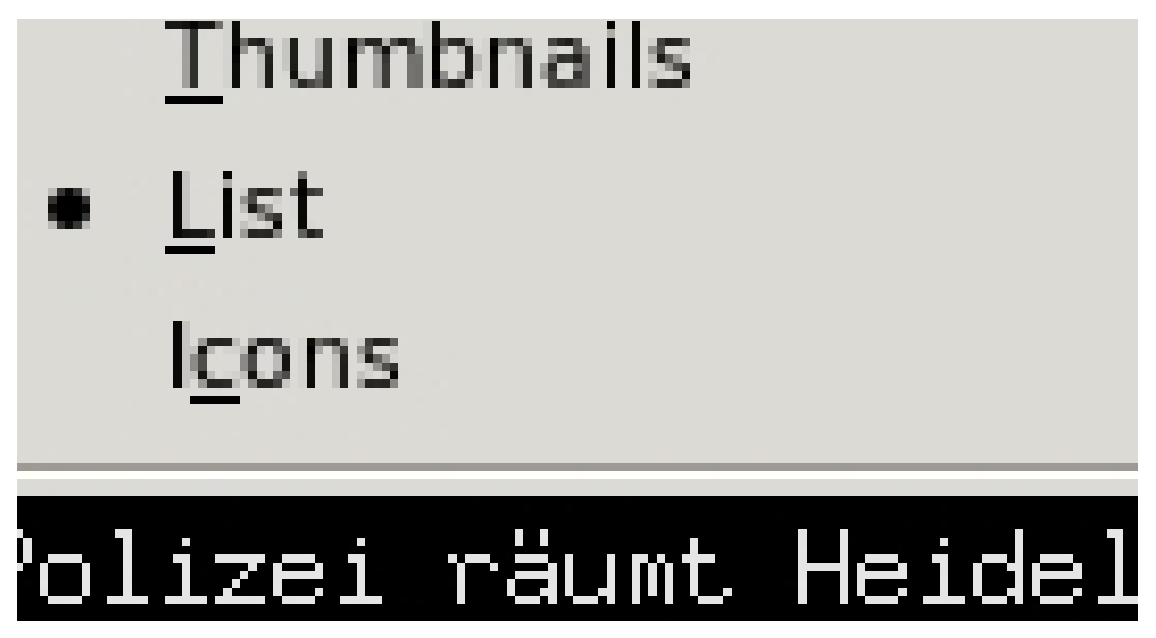
\includegraphics[width=.5\textwidth]{xft.eps}
\begin{list}{$\bullet$}{\itemsep=.1em}
        \item Verschiedene APIs fürs Rendern von Text: X Core Fonts und xft
        \item xft = X FreeType, antialiased fonts, Pango, GTK
        \item Problem mit X Core Fonts: keine Sonderzeichen
        \item …oder? \texttt{misc-fixed-*-iso10646}, also X Core Fonts mit Universal Character Set (= Unicode-Zeichen). Nicht 100\% vollständig
        \item urxvt: benutzt beide APIs, pro Glyph unterschiedlich
        \item Trend geht leider zu fontconfig/xft :-(
\end{list}
\end{slide}

\begin{slide}[method=direct]{Umlaute und Sonderzeichen (2)}
\begin{list}{$\bullet$}{\itemsep=.5em}
        \item X hat eigenes Encoding: Compound Text
        \item Früher ICCCM (Compound text, z.B. Atom WM\_NAME)\\
        ICCCM = Inter-Client Communication Conventions Manual
        \item heute EWMH (UTF-8, z.B. Atom \_NET\_WM\_NAME)\\
        EWMH = Extended Window Manager Hints (= NetWM)
        \item XImageText16 (bzw xcb\_image\_text\_16) erwartet UCS-2\\
        $\Rightarrow$ \texttt{iconv\_open(UCS2\_BE, UTF-8)}
\end{list}
\isrc{i3/src/util.c:191ff, i3/src/handlers.c:663ff}
\end{slide}


\begin{slide}[method=direct]{Colorpixel}
\begin{list}{$\bullet$}{\itemsep=.5em}
        \item Heutzutage: TrueColor. Früher: 8 bit o.ä.
        \item Colormaps: Geben an welche Farben die Hardware kann
        \item Colorpixel: Ein Wert aus der Colormap, der der gewünschten Farbe am nähesten kommt
        \item Bei TrueColor: \texttt{return (red << 16) + (green << 8) + blue;}
        \item Alles andere: Round-Trip zum X-Server:
\end{list}
\begin{code}
        #define RGB_8_TO_16(i) (65535 * ((i) & 0xFF) / 255)
        xcb_alloc_color_reply_t *reply;
        reply = xcb_alloc_color_reply(conn, xcb_alloc_color(conn,
                root_screen->default_colormap, RGB_8_TO_16(red),
                RGB_8_TO_16(green), RGB_8_TO_16(blue)), NULL);
        if (!reply)
                die("Could not allocate color\n");
        return reply->pixel;
\end{code}
\isrc{i3/src/xcb.c:76ff}
\end{slide}

\begin{slide}[method=direct]{Hints}
\begin{list}{$\bullet$}{\itemsep=.5em}
        \item NetWM
        \begin{description}
                \item[NET\_WM\_WINDOW\_TYPE] dock, dialog, utility, toolbar, splashscreen
                \item[NET\_WM\_NAME] Fenstertitel (UTF-8), auch auf dem root-Fenster
                \item[NET\_WM\_STRUT\_PARTIAL] Reservierter Bereich am Bildschirmrand (Docks), z.B. für dzen2
        \end{description}
        \item ICCCM
        \begin{description}
                \item[WM\_NAME] Fenstertitel (Compound Text)
                \item[WM\_TRANSIENT\_FOR] Zugehöriges, "`temporäres"' Fenster für Anwendung X ($\Rightarrow$ floating)
                \item[WM\_CLASS] Fensterklasse (z.B. "`urxvt"'), praktisch zum identifizieren
                \item[WM\_NORMAL\_HINTS] (Size hints), beinhaltet Aspect Ratio (mplayer!), minimale und maximale Größe
        \end{description}
\end{list}
\end{slide}

\begin{slide}[method=direct]{Hints (2)}
\begin{code}
int handle_transient_for(void *data, xcb_connection_t *conn,
           uint8_t state, xcb_window_t window,
           xcb_atom_t name, xcb_get_property_reply_t *reply)
{
  xcb_window_t transient_for;
  if (reply != NULL) {
    if (!xcb_get_wm_transient_for_from_reply(&transient_for, reply)) {
      LOG("Not transient for any window\n");
      return 1;
    }
  } else {
    if (!xcb_get_wm_transient_for_reply(conn,
        xcb_get_wm_transient_for_unchecked(conn, window),
        &transient_for, NULL)) {
      LOG("Not transient for any window\n");
      return 1;
    }
  }
  if (client->floating == FLOATING_AUTO_OFF)
    toggle_floating_mode(conn, client, true);
  return 1;
}
\end{code}
\end{slide}

\begin{slide}[method=direct]{Gotchas}
\begin{list}{$\bullet$}{\itemsep=.5em}
        \item Flushing (\texttt{xcb\_flush(connection);})
        \item \texttt{WM\_STATE} != \texttt{WM\_STATE\_NORMAL}
        \item Eventloops / Caching von xcb (GIMP splash screen)
\end{list}
\end{slide}


\begin{slide}{Zusammenfassung}
\begin{list}{$\bullet$}{\itemsep=.5em}
        \item Bindings aufsetzen, Eventmask konfigurieren
        \item Events/Hints abarbeiten
        \item Decorations zeichnen
\end{list}
\end{slide}

\begin{slide}{Lust bekommen?}
\begin{list}{$\bullet$}{\itemsep=1em}
        \item git clone \url{git://code.stapelberg.de/i3}
        \item development branch: \texttt{git checkout --track -b next origin/next}
        \item Debian: \texttt{apt-get install i3-wm/unstable}
        \item non-Debian: \texttt{cd i3; cat DEPENDS; make \&\& sudo make install}
        \item in \~{}/.xsession: \texttt{exec /usr/bin/i3}
        \item Siehe manpage \texttt{i3(1)}, user’s guide, how to hack
\end{list}
\end{slide}

\begin{slide}{exit(0);}
\begin{list}{$\bullet$}{\itemsep=1em}
        \item git-webinterface: \url{http://code.stapelberg.de/git/i3}
        \item Website: \url{http://i3.zekjur.net}
        \item IRC: \#i3 auf irc.twice-irc.de
        \item xcb: \url{http://xcb.freedesktop.org/}
        \item 50-Zeilen-WM: \url{http://incise.org/tinywm.html}
        \item „Why X is not our ideal window system”: \url{http://www.std.org/~msm/common/WhyX.pdf}
        \item …noch Fragen?
\end{list}
\end{slide}

\end{document}
